
\title{Sistemi Informativi \\ Laboratorio 7}
\author{
        Catalin Copil
            \and
        Mattia de Stefani
            \and
        Giulio Lovisotto
}
\date{\today}

\documentclass[12pt]{article}
\usepackage{algorithmicx}
\usepackage{algpseudocode}
\usepackage{geometry}
\usepackage{graphicx}
\usepackage{caption}
\usepackage{subcaption}

\addtolength{\topmargin}{-.5in}
\begin{document}
\maketitle

\section{Descrizione}
La nostra funzione di reperimento utilizzera' i primi $N$ documenti prodotti da BM25 per costruire il grafo delle citazioni $R_q$, tale grafo verra' espanso per ottenere un grafo allargato $B_q$, e su quest'ultimo verra' calcolato \textsc{hits}. La funzione combinera' poi gli score di BM25 ($sc$) con i punteggi di authority ($auth$) e hubbiness ($hub$) per i primi $N$ documenti, e li riordinera' per $hits_{score}$ decrescente:

\[ hits_{score} =  \alpha \cdot sc + \beta \cdot auth + \gamma \cdot hub,\]

$\alpha$ varia in [0, 1],  mentre $\beta, \gamma$ sono parametri che possono variare tra [-1, 1], in quanto vogliamo cogliere possibili influenze negative sul di tali valori. Nella precedente funzione i valori di $sc, auth, hub$ vengono normalizzati in [0, 1] prima del calcolo. 

 Vogliamo provare diverse combinazioni di tali valori per ottenere la massima precisione.



\section{Risultati}

Abbiamo studiato la relazione tra il grafo radice $R_q$ e il grafo allargato $B_q$ per capire le dinamiche dell'espansione. Per esempio Figura \ref{fig:unodue} riportano i tali grafi per la query $56$.
\begin{figure}
	\centering
	\begin{subfigure}{.5\textwidth}
		\centering
		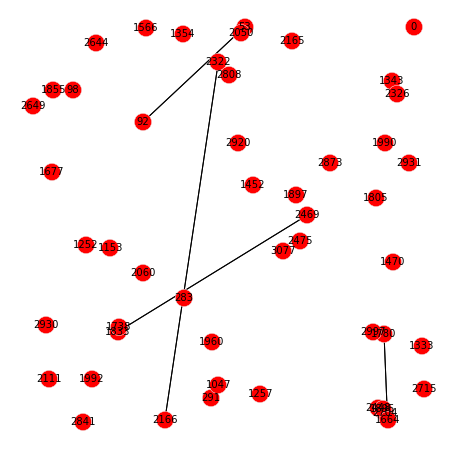
\includegraphics[width=1\textwidth]{../R.png}
		\caption{Grafo radice ($R_{56}$)}
		\label{fig:uno}
	\end{subfigure}%
	\begin{subfigure}{.5\textwidth}
		\centering
		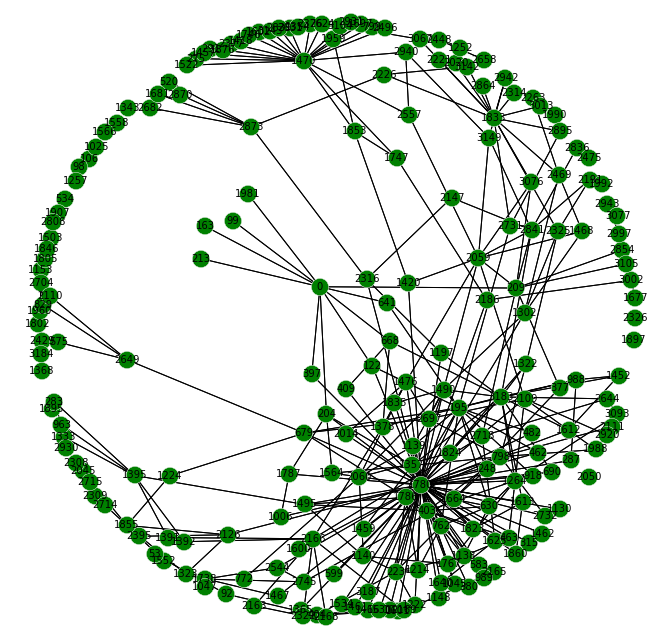
\includegraphics[width=1\textwidth]{../B.png}
		\caption{Grafo base ($B_{56}$).}
		\label{fig:due}
	\end{subfigure}
	\caption{Grafi ottenuti applicando \textsc{hits} sui top $N=50$ documenti per la query $56$.}
	\label{fig:unodue}
\end{figure}
Abbiamo scelto per i parametri $\alpha, \beta, \gamma$ i valori $1.0, 0.1, 0.1$, mentre per $N$ abbiamo usato il valore $50$. Abbiamo ottenuto la $map$ riportata in Figura \ref{fig:tre}:
\begin{figure}[htbp]
	\begin{center}
		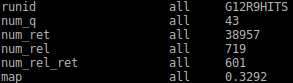
\includegraphics[width=0.9\textwidth]{../snapshot2.png}
		\caption{Mean Average Precision utilizzando \textsc{hits} nella funzione di reperimento.}
		\label{fig:tre}
	\end{center}
\end{figure}

\bibliographystyle{abbrv}
\bibliography{main}
\end{document}